\documentclass[11pt]{article}
\usepackage[margin=0.9in]{geometry}
\usepackage[T1]{fontenc}
\usepackage{lmodern}
\usepackage{amsmath,amssymb}
\usepackage{booktabs,tabularx,array,multirow}
\usepackage{enumitem}
\usepackage{xcolor}
\usepackage{graphicx}
\usepackage{float}
\usepackage{caption}
\usepackage{textcomp}
\usepackage[colorlinks=true,linkcolor=blue!50!black,citecolor=blue!50!black,urlcolor=blue!50!black]{hyperref}

\setlist{itemsep=1pt,topsep=3pt,parsep=0pt}
\captionsetup{font=small,labelfont=bf}
\newcolumntype{L}{>{\raggedright\arraybackslash}X}
\graphicspath{{generated/}{./}}
% ---- begin generated/numbers.tex (generated from results/*.json) ----
\newcommand{\TotSOne}{0.94}
\newcommand{\SrvSOne}{0.85}
\newcommand{\TotSTwo}{0.54}
\newcommand{\SrvSTwo}{0.45}
\newcommand{\CliS}{89}
\newcommand{\UpS}{3.81}
\newcommand{\DownS}{0.93}
\newcommand{\CommS}{4.7}
\newcommand{\PreS}{2.2}
\newcommand{\FinalS}{14}
\newcommand{\SlowPlainS}{12,669}
\newcommand{\BytesPlainS}{475}
\newcommand{\BytesKanonS}{2}
\newcommand{\KanonDownS}{2.43 MB}
\newcommand{\RunsS}{10}
\newcommand{\TPS}{320}
\newcommand{\FPS}{0}
\newcommand{\FNS}{0}
\newcommand{\LerrS}{0}
\newcommand{\TotMOne}{3.13}
\newcommand{\SrvMOne}{2.99}
\newcommand{\TotMTwo}{1.71}
\newcommand{\SrvMTwo}{1.56}
\newcommand{\CliM}{136}
\newcommand{\UpM}{3.81}
\newcommand{\DownM}{8.50}
\newcommand{\CommM}{12.3}
\newcommand{\PreM}{33.6}
\newcommand{\FinalM}{14}
\newcommand{\SlowPlainM}{19,025}
\newcommand{\BytesPlainM}{1,233}
\newcommand{\BytesKanonM}{5}
\newcommand{\KanonDownM}{2.41 MB}
\newcommand{\RunsM}{10}
\newcommand{\TPM}{320}
\newcommand{\FPM}{0}
\newcommand{\FNM}{0}
\newcommand{\LerrM}{0}
\newcommand{\TotLOne}{5.75}
\newcommand{\SrvLOne}{5.54}
\newcommand{\TotLTwo}{3.03}
\newcommand{\SrvLTwo}{2.83}
\newcommand{\CliL}{208}
\newcommand{\UpL}{10.63}
\newcommand{\DownL}{9.84}
\newcommand{\CommL}{20.5}
\newcommand{\PreL}{34.6}
\newcommand{\FinalL}{31}
\newcommand{\SlowPlainL}{27,854}
\newcommand{\BytesPlainL}{2,050}
\newcommand{\BytesKanonL}{8}
\newcommand{\KanonDownL}{2.41 MB}
\newcommand{\RunsL}{10}
\newcommand{\TPL}{320}
\newcommand{\FPL}{0}
\newcommand{\FNL}{0}
\newcommand{\LerrL}{0}
\newcommand{\CPU}{Intel Xeon Processor @ 2.30GHz}
\newcommand{\HWThreads}{2}
% ---- end generated/numbers.tex ----
% primitive input: expandable inside tabular (needed for \midrule in snippets)
\makeatletter\newcommand{\tabin}[1]{\@@input #1 }\makeatother

% ---- EDIT THIS: public URL of your GitHub repository ----
\newcommand{\repourl}{\url{https://github.com/YOUR-USERNAME/breachcheck-psi}}

\title{Encrypted Compromised-Credential Checking via Homomorphic-Encryption-Based Unbalanced Private Set Intersection\\[2pt]
\large CYB 599 Graduate Project --- Part 3: Implementation and Evaluation}
\author{Bhanu Aniruth Pasala}
\date{November 16, 2026}

\begin{document}
\maketitle
\vspace{-1.6em}


\section{What Was Built}
The repository implements the Part~2 protocol end to end in C++17: a verifiable OPRF, signed parameter manifest, cuckoo/simple hashing, BFV-based labeled PSI with depth-1 windowed evaluation, rerandomization and noise flooding, bit-packed responses, and client decoding with label integrity checks. Table~\ref{tab:arch} maps each component to the design element it implements.

\begin{table}[H]
\centering\footnotesize
\caption{Implementation map (all paths relative to the repository root).}
\label{tab:arch}
\begin{tabularx}{\textwidth}{@{}p{3.0cm}p{3.4cm}Lp{2.3cm}@{}}
\toprule
Component & Files & Part~2 design element & Library \\
\midrule
VOPRF + batched DLEQ & \texttt{src/oprf.*} & 2HashDH OPRF (RFC~9497 ristretto255-SHA512), Chaum--Pedersen proof & libsodium 1.0.22 \\
Signed manifest & \texttt{src/manifest.*} & Ed25519 over params, $pk_S$, table seed, $n_{\max}$, DB version; client pinning & libsodium \\
Item derivation, hashing & \texttt{src/hashing.*} & 100-bit $\hat o$ in 5$\times$20-bit felts, 100-bit label pad, 3-way cuckoo & --- \\
Polynomials over $\mathbb{Z}_t$ & \texttt{src/zt.*} & Roots polynomial $P$, Newton interpolation $L$ (Barrett reduction) & --- \\
Server & \texttt{src/server.*} & Collision-aware partitions, window powers, $r_p\odot P$, flooding, mod-switch & SEAL 4.1.2 (BFV) \\
Client & \texttt{src/client.*} & Padding to 256, fresh keys per session, zero test, $0^{52}$ label check & SEAL 4.1.2 \\
Wire format & \texttt{src/protocol.*} & Seeded SEAL objects (upload); 56/60-bit packed ciphertexts (download) & SEAL \\
Baselines & \texttt{src/baseline.*} & Plaintext lookup; HIBP-style $k$-anonymity prefix buckets & --- \\
\bottomrule
\end{tabularx}
\end{table}

\paragraph{Deviations from the Part~2 design.} (1) SEAL serializes coefficients as 64-bit words (compression disabled to avoid extra dependencies), so the upload is 3.81\,MB rather than the 3.31\,MB bit-packed estimate. The response uses a custom 56-bit packing and matches the estimate exactly (8.49\,MB). (2) Collision-aware partitioning needs a fallback partition, so $\alpha\ge2$ is enforced (this affects only the $n=2^{12}$ test set; Section~\ref{sec:tests}). (3) The flooding width is a fixed public parameter, $b=132$ bits for $N=8192$, calibrated from the measured evaluation noise and including the $\log_2 N$ smudging term the design omitted (Section~\ref{sec:noise}). (4) The 2-thread server parallelizes across partitions, as planned. (5) Rate-limit tokens and TLS are not implemented: client and server exchange serialized byte strings in one process.

\section{Experimental Setup}
All measurements ran on a cloud VM with an \CPU\ (\HWThreads\ vCPUs, 7.8\,GB RAM), Ubuntu 24.04, GCC 13.3 (\texttt{-O3 -march=native}), SEAL 4.1.2 without Intel HEXL, and libsodium 1.0.22. Server records are synthetic and deterministic: each is the SHA-256 of a normalized username/password pair with a random 48-bit label. Every query uses a fresh client set of 256 credentials containing 32 planted breached credentials. The timed runs per set and thread count are 5 repetitions after one warm-up; we report medians and interquartile ranges. A separate, untimed instrumented run records noise budgets using \texttt{NoiseProbe}, which hands the \emph{client's} decryptor to the measurement code only. Sizes are the exact byte lengths of the serialized messages. Network time is modelled (Section~\ref{sec:baseline}), not measured. To check reproducibility, a fresh copy of the repository (no build directory or results) ran \texttt{./run.sh quick} unattended: it cloned SEAL v4.1.2 and libsodium 1.0.22 from GitHub, compiled them, and passed all tests and the demo.

\section{Correctness Tests}\label{sec:tests}
\texttt{build/bcpsi\_tests} runs 19 tests with 4{,}523 assertions (\texttt{results/tests\_full.log}); all pass. Table~\ref{tab:tests} summarizes them.
\begin{table}[tbp]
\centering\footnotesize
\caption{Correctness and security-property tests (all passing).}
\label{tab:tests}
\begin{tabularx}{\textwidth}{@{}p{4.6cm}L@{}}
\toprule
Test & What is checked / observed result \\
\midrule
RFC 9497 conformance & \texttt{DeriveKeyPair}, \texttt{Blind}, \texttt{BlindEvaluate}, \texttt{Finalize} and \emph{batched} proofs (fixed $r$) reproduce the RFC's ristretto255-SHA512 vectors byte-for-byte, OPRF and VOPRF modes \\
DLEQ soundness & Client rejects: wrong committed key, one output under a different key (key partitioning), forged $s$, reordered outputs; server rejects invalid group elements \\
$\mathbb{Z}_t$ arithmetic & Inverse table; $P$ vanishes exactly on its roots; $L$ interpolates 50 random sets of up to 63 points \\
Parameters & $\alpha$, overflow $\le2^{-40}$, false-positive bound $\le2^{-40}$, $t\equiv1 \bmod 2N$, $\log q$ within HE-Standard limits \\
Cuckoo hashing & 2{,}000 tables of 256 items in 1638 bins: 0 failures, at most 7 evictions \\
Manifest & Bad signature, wrong signer and mismatched pinned parameters are all rejected \\
End-to-end scenarios & 1, 20 and 256 items with 0, 1, 8, 32, 256 members: exact intersection, all labels correct \\
Multi-partition ($n=2^{16}$, $\alpha=4$) & 3 queries $\times$ 64 members: 192/192 found, 0 false positives, 0 label errors \\
False positives & 40 queries $\times$ 256 non-members $=$ 10{,}240 probes: \textbf{0} false positives (bound: $2^{-57}$ per query) \\
Tampered labels & Server adds 1 to every label slot: all 16 hits detected by the 52-bit check \\
Malformed input & Wrong ciphertext count, truncated or out-of-range ciphertext, wrong object type, ciphertext from another parameter set, wrong OPRF batch size, truncated or out-of-range response: all rejected \\
Fixed shape & Client sets $(m,k)\in\{(1,0),(1,1),(100,50),(256,0),(256,256)\}$: identical upload/download bytes and identical operation counts (49 ct$\times$ct, 143 pt$\times$ct on the test set) \\
Noise & Final budget $\ge5$ bits with $b=132$ (measured: 14 bits) \\
Masking & Decrypted non-matching slots of $R_p$ uniform over $\mathbb{Z}_t$: $\chi^2_{63}\in[53,89]$ over four independent runs (critical value 110 at $p=10^{-4}$), at most 2 zero slots of 8190 (expected $\approx$0.5) \\
Baselines & Plaintext and $k$-anonymity baselines return the same intersection and labels \\
\bottomrule
\end{tabularx}
\end{table}

\noindent Writing these tests caught one real design gap, and the scaling run caught a second (an $\alpha$-derivation bug at $n=2^{22}$, now covered by a regression test): with a single partition ($\alpha=1$), a 20-bit felt collision ($\approx$0.2--0.4 expected per $2^{12}$ records) has no other partition to go to and preprocessing aborts. The fix is $\alpha\ge2$. Across all benchmark runs (\RunsS{} per set, $\times$32 members) every planted credential was found with the correct label: \TPS/\TPS, \TPM/\TPM\ and \TPL/\TPL\ for S, M, L, with \FPM{} false positives.

\section{Performance}

\subsection{Parameter sets}
We evaluate three sets (Table~\ref{tab:params}). S and M share the Part~2 ring ($N=8192$, $\log q=218$) and differ in $n$. L doubles the ring at $n=2^{20}$ to isolate the effect of ring size. All sets use $d=63$, a base-8 two-digit window (14 query ciphertexts), $m=256$ and 48-bit labels.
\begin{table}[H]
\centering\small
\caption{Parameter sets. $\alpha$ is derived from the binomial overflow bound; FP is the per-query false-positive bound $m\alpha(d/t)^5$.}
\label{tab:params}
\begin{tabular}{@{}lrrrrrrrrrr@{}}
\toprule
Set & $n$ & $N$ & $\log q$ (data) & $t$ & $B$ & $\alpha$ & $C=\alpha d$ & flood $b$ & overflow & FP \\
\midrule
% ---- begin generated/tab_params.tex (generated from results/*.json) ----
S & $2^{16}$ & 8192 & 218 (168) & 1,097,729 & 1638 & 4 & 252 & 132 & $2^{-74}$ & $2^{-60}$ \\
M & $2^{20}$ & 8192 & 218 (168) & 1,097,729 & 1638 & 37 & 2331 & 132 & $2^{-53}$ & $2^{-57}$ \\
L & $2^{20}$ & 16384 & 300 (240) & 1,146,881 & 3276 & 20 & 1260 & 170 & $2^{-55}$ & $2^{-58}$ \\
% ---- end generated/tab_params.tex ----
\bottomrule
\end{tabular}
\end{table}

\subsection{Server preprocessing}
\begin{table}[H]
\centering\small
\caption{Offline preprocessing on 2 threads (seconds), maximum bin load vs.\ capacity, felt collisions resolved by moving an item to a later partition, and resident database size.}
\label{tab:pre}
\begin{tabular}{@{}lrrrrrrrr@{}}
\toprule
Set & OPRF & binning & polynomials & encode & total & max load / $C$ & collisions & DB (MB) \\
\midrule
% ---- begin generated/tab_pre.tex (generated from results/*.json) ----
S & 1.7 & 0.0 & 0.4 & 0.0 & \textbf{2.2} & 157/252 & 25 & 39 \\
M & 27.9 & 0.3 & 4.9 & 0.5 & \textbf{33.6} & 2077/2331 & 482 & 482 \\
L & 27.9 & 0.5 & 5.3 & 0.8 & \textbf{34.6} & 1108/1260 & 461 & 658 \\
% ---- end generated/tab_pre.tex ----
\bottomrule
\end{tabular}
\end{table}
Preprocessing is dominated by the $n$ OPRF evaluations: 27\,\textmu s each in wall-clock time, i.e.\ 53\,\textmu s of CPU per evaluation on two threads (Table~\ref{tab:pre}). The measured maximum bin load (2077 of 2331 at $n=2^{20}$) confirms the overflow analysis has slack. The resident database is 482\,MB at $n=2^{20}$: 78\,MB of raw $P$ coefficients plus 404\,MB of label plaintexts kept in NTT form. Part~2 estimated 0.54\,GB.

\subsection{Online computation time}
\begin{figure}[H]
\centering
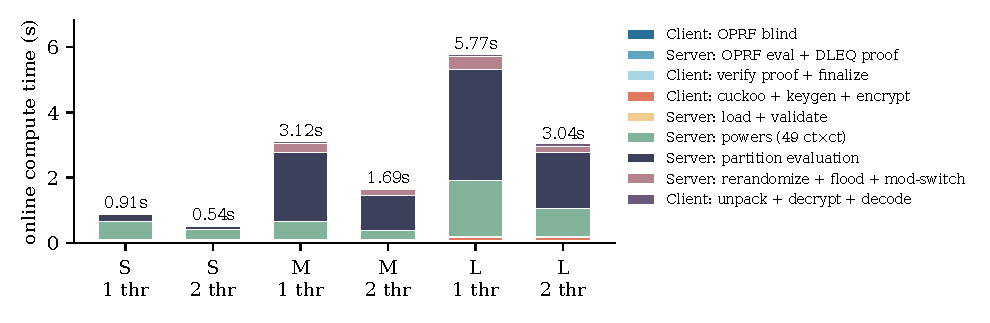
\includegraphics[width=\textwidth]{fig_time.pdf}
\vspace{-1.2em}
\caption{Median online compute time per query by stage (no network). The server's partition evaluation and power computation dominate. Client work is under 0.21\,s in every setting.}
\label{fig:time}
\end{figure}
\begin{table}[H]
\centering\small
\caption{Median online time per stage in milliseconds (5 runs each). Columns: set / threads.}
\label{tab:time}
\setlength{\tabcolsep}{4.5pt}\footnotesize
\begin{tabular}{@{}lrrrrrr@{}}
\toprule
 & \multicolumn{2}{c}{S} & \multicolumn{2}{c}{M} & \multicolumn{2}{c}{L} \\
\cmidrule(lr){2-3}\cmidrule(lr){4-5}\cmidrule(lr){6-7}
Stage & 1 thr & 2 thr & 1 thr & 2 thr & 1 thr & 2 thr \\
\midrule
% ---- begin generated/tab_time.tex (generated from results/*.json) ----
Client: OPRF blind & 13.5 & 12.9 & 13.1 & 13.2 & 13.1 & 13.1 \\
Server: OPRF eval + DLEQ proof & 25.3 & 23.5 & 23.5 & 23.6 & 23.6 & 23.7 \\
Client: verify proof + finalize & 37.3 & 37.7 & 36.9 & 36.9 & 36.9 & 37.0 \\
Client: cuckoo + keygen + encrypt & 32.0 & 31.4 & 31.4 & 30.5 & 88.0 & 84.6 \\
Server: load + validate & 11.7 & 11.9 & 12.0 & 11.6 & 35.5 & 33.0 \\
Server: powers (49 ct$\times$ct) & 532 & 299 & 550 & 283 & 1,719 & 857 \\
Server: partition evaluation & 220 & 106 & 2,112 & 1,067 & 3,401 & 1,713 \\
Server: rerandomize + flood + mod-switch & 31.0 & 16.6 & 285 & 164 & 381 & 205 \\
Client: unpack + decrypt + decode & 6.1 & 5.9 & 54.7 & 56.3 & 69.5 & 71.2 \\
\midrule
Server total & 848 & 454 & 2,994 & 1,563 & 5,541 & 2,827 \\
Client total & 89.0 & 89.9 & 136 & 144 & 208 & 205 \\
\textbf{Compute total} & \textbf{937} & \textbf{544} & \textbf{3,129} & \textbf{1,707} & \textbf{5,749} & \textbf{3,032} \\
\quad server IQR & 805--876 & 448--485 & 2,879--3,118 & 1,505--1,635 & 5,410--5,574 & 2,806--2,948 \\
% ---- end generated/tab_time.tex ----
\bottomrule
\end{tabular}
\end{table}
Server time scales with the number of partitions: partition evaluation costs about 57\,ms per partition on one thread at $N=8192$ (encode $r_p\odot c_{p,e}$, then 63+62 NTT-domain plaintext multiplications). The fixed cost of 49 ciphertext multiplications with relinearization is $\approx$0.55\,s. Two threads give a $1.9\times$ server speedup. Within partition evaluation, re-encoding the randomized coefficients $r_p\odot c_{p,e}$ takes 47\% of the CPU time (968 of 2075\,ms for M) and the plaintext multiplications the rest. Client work is small and nearly constant: the 256-element VOPRF (50\,ms in total, 27\,ms of it proof verification), key generation and 14 encryptions (31\,ms at $N=8192$), and unpacking plus decryption (55\,ms). Doubling the ring (L) costs $1.8\times$ more server time than M even though $\alpha$ drops from 37 to 20, because each operation touches $2\times$ the slots and $4/3\times$ the RNS primes.

\subsection{Scaling in the database size}
\begin{table}[H]
\centering\small
\caption{Scaling on the $N=8192$ ring: $\alpha$, preprocessing (s, 2 threads), database (MB), server online time (s, 1 and 2 threads), response ciphertexts, total communication.}
\label{tab:scale}
\begin{tabular}{@{}rrrrrrrr@{}}
\toprule
$n$ & $\alpha$ & preprocess & DB & server 1 thr & server 2 thr & resp.\ cts & comm. \\
\midrule
% ---- begin generated/tab_scale.tex (generated from results/*.json) ----
$2^{16}$ & 4 & 2 & 39 & 0.85 & 0.45 & 8 & 4.74 MB \\
$2^{20}$ & 37 & 34 & 482 & 2.99 & 1.56 & 74 & 12.31 MB \\
$2^{22}$ & 134 & 137 & 1834 & 9.14 & 4.68 & 268 & 34.56 MB \\
% ---- end generated/tab_scale.tex ----
\bottomrule
\end{tabular}
\end{table}
Cost is affine in the number of partitions, $\alpha\approx 3n/(Bd)$ plus a few percent of slack (Table~\ref{tab:scale}). A least-squares fit over the three sizes gives a server time of $0.61\,\mathrm{s}+64\,\mathrm{ms}\cdot\alpha$ on one thread, which predicts S, M and the $2^{22}$ point to within 2.2\%. Preprocessing (34\,s$\to$137\,s) and memory (0.48$\to$1.83\,GB) grow linearly with $n$, and every query at $2^{22}$ was again answered correctly. Upload stays at 3.81\,MB whatever $n$ is; the download grows by 230\,KB per partition (two packed ciphertexts).

\subsection{Communication, ciphertext and proof sizes}
\begin{figure}[H]
\centering
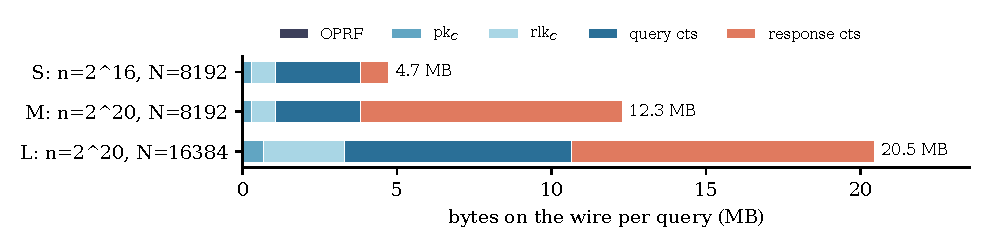
\includegraphics[width=\textwidth]{fig_comm.pdf}
\vspace{-1.4em}
\caption{Bytes per query. Upload is constant in $n$; download is $2\alpha$ response ciphertexts.}
\label{fig:comm}
\end{figure}
\begin{table}[H]
\centering\small
\caption{Message and object sizes (identical in every run: the protocol has a fixed shape). The DLEQ proof is 64\,B for all 256 evaluations; the Ed25519 manifest signature is 64\,B.}
\label{tab:size}
\begin{tabular}{@{}llrrr@{}}
\toprule
Object & dir. & S & M & L \\
\midrule
% ---- begin generated/tab_size.tex (generated from results/*.json) ----
OPRF request ($256\times32$ B) & up & 8.2 KB & 8.2 KB & 8.2 KB \\
OPRF response + DLEQ proof (64 B) & down & 8.3 KB & 8.3 KB & 8.3 KB \\
Public key $pk_C$ (seeded) & up & 262.3 KB & 262.3 KB & 655.6 KB \\
Relinearization keys $rlk_C$ (seeded) & up & 787.1 KB & 787.1 KB & 2.62 MB \\
Query: 14 ciphertexts (seeded) & up & 2.76 MB & 2.76 MB & 7.34 MB \\
Response: $2\alpha$ ciphertexts (bit-packed) & down & 917.5 KB & 8.49 MB & 9.83 MB \\
\midrule
One query ciphertext & up & 196.8 KB & 196.8 KB & 524.5 KB \\
One response ciphertext & down & 114.7 KB & 114.7 KB & 245.8 KB \\
\midrule
\textbf{Total upload} & & \textbf{3.81 MB} & \textbf{3.81 MB} & \textbf{10.63 MB} \\
\textbf{Total download} & & \textbf{925.8 KB} & \textbf{8.50 MB} & \textbf{9.84 MB} \\
% ---- end generated/tab_size.tex ----
\bottomrule
\end{tabular}
\end{table}
The proof machinery is nearly free: one 64-byte batched DLEQ proof covers all 256 OPRF evaluations, and verifying it costs the client $\approx$27\,ms. The client's fresh $pk_C$ and $rlk_C$ (1.05\,MB at $N=8192$) are 27\% of the upload. They are the price of unlinkable sessions (Part~2 leakage analysis). Mod-switching each response ciphertext to one 56-bit prime and bit-packing it shrinks it from 393\,KB at the top level to 115\,KB.

\subsection{Noise budget and flooding}\label{sec:noise}
\begin{table}[H]
\centering\small
\caption{Measured invariant noise budget (bits, minimum over all ciphertexts) after each server stage, and the resulting statistical circuit-privacy parameter.}
\label{tab:noise}
\begin{tabular}{@{}lrrr@{}}
\toprule
Stage & S & M & L \\
\midrule
% ---- begin generated/tab_noise.tex (generated from results/*.json) ----
Fresh query ciphertext & 143 & 143 & 215 \\
After powers (depth 1) & 111 & 111 & 182 \\
After partition evaluation & 84 & 83 & 154 \\
After rerandomize + flood & 14 & 14 & 48 \\
After mod-switch to $q_0$ (sent) & 14 & 14 & 31 \\
\midrule
Flooding width $b$ (bits) & 132 & 132 & 170 \\
Statistical parameter $\lambda=b-\log_2 E_{\mathrm{eval}}-\log_2 N$ & 56 & 55 & 91 \\
% ---- end generated/tab_noise.tex ----
\bottomrule
\end{tabular}
\end{table}
\begin{figure}[H]
\centering
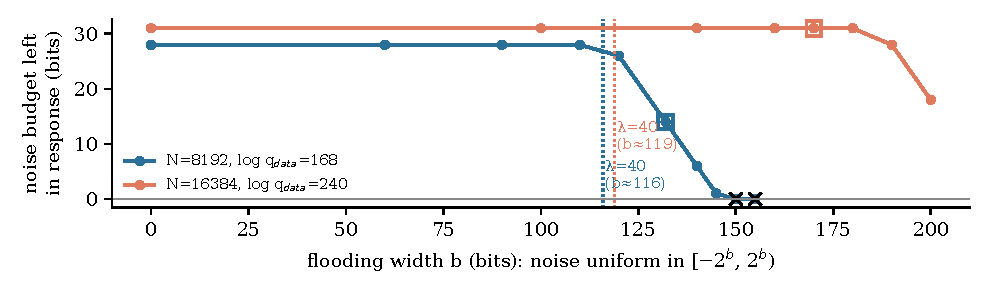
\includegraphics[width=\textwidth]{fig_flood.pdf}
\vspace{-1.4em}
\caption{Flooding sweep (3 queries per point). Squares: chosen widths. Crosses: decryption failed. Dotted lines: smallest width giving $\lambda=40$.}
\label{fig:flood}
\end{figure}
Table~\ref{tab:noise} confirms the depth-1 design: one ciphertext multiplication costs 32 bits and the plaintext products 27 more, leaving 84 bits before flooding (Part~2 estimated 68). The evaluated noise is $E\approx 2^{168-20-84-1}=2^{63}$, so flooding $c_0$ with uniform noise in $[-2^{b},2^{b})$ gives statistical distance at most $N\cdot E/2^{b}$, i.e.\ $\lambda=b-63-13$. The sweep in Figure~\ref{fig:flood} shows that $N=8192$ supports at most $b\approx145$ and that $\lambda=40$ needs $b\ge116$. We chose $b=132$ ($\lambda\approx56$), which leaves 14 bits of noise margin. For $N=16384$, $b=170$ gives $\lambda\approx91$ with no loss of budget, so L could afford a deeper circuit (larger $d$, fewer partitions).

\subsection{Design budget vs.\ measurement (set M)}
\begin{center}\small
\begin{tabular}{@{}lrr@{}}
\toprule
Quantity & Part 2 estimate & Measured \\
\midrule
Upload / download & 3.31 / 8.50 MB & 3.81 / 8.50 MB \\
Server online compute (1 thread) & 2.01 s & \SrvMOne\ s \\
Client compute & 0.15 s & 0.14 s \\
Online total incl.\ 50 Mbit/s link + 2 RTT (1 / 2 threads) & 4.2 / 2.8 s & 5.2 / 3.8 s \\
Noise budget left in response & $\approx$20 bits & 14 bits \\
Server database in memory & 0.54 GB & 0.48 GB \\
\bottomrule
\end{tabular}
\end{center}
The Part~2 per-operation timing assumptions were optimistic by about $1.5\times$ for this VM (ct$\times$ct with relinearization measured $\approx$11\,ms, not 4\,ms). As a result the $<5$\,s target is met with two server threads but missed by 0.2\,s on one.

\section{Comparison to Non-Private Baselines}\label{sec:baseline}
\begin{table}[H]
\centering\small
\caption{Same data and 256-credential client sets. Time is total compute per query (HE-uPSI: 2 threads). The last column is the number of bits of each queried credential hash revealed to the server.}
\label{tab:baseline}
\begin{tabular}{@{}llrrr@{}}
\toprule
Set & Scheme & Time & Up / Down & Bits revealed \\
\midrule
% ---- begin generated/tab_baseline.tex (generated from results/*.json) ----
\multirow{3}{*}{S} & Plaintext lookup & 43\,\textmu s & 8.2 KB / 1.8 KB & 256 (full hash) \\
 & $k$-anon.\ prefix (8 bits) & 437\,\textmu s & 256 B / 2.43 MB & 8 \\
 & This work (HE-uPSI) & 0.54\,s & 3.81 MB / 925.8 KB & 0 \\
\midrule
\multirow{3}{*}{M} & Plaintext lookup & 90\,\textmu s & 8.2 KB / 1.8 KB & 256 (full hash) \\
 & $k$-anon.\ prefix (12 bits) & 1135\,\textmu s & 512 B / 2.41 MB & 12 \\
 & This work (HE-uPSI) & 1.71\,s & 3.81 MB / 8.50 MB & 0 \\
\midrule
\multirow{3}{*}{L} & Plaintext lookup & 109\,\textmu s & 8.2 KB / 1.8 KB & 256 (full hash) \\
 & $k$-anon.\ prefix (12 bits) & 1376\,\textmu s & 512 B / 2.41 MB & 12 \\
 & This work (HE-uPSI) & 3.03\,s & 10.63 MB / 9.84 MB & 0 \\
% ---- end generated/tab_baseline.tex ----
\bottomrule
\end{tabular}
\end{table}
Privacy is expensive in computation and cheap in round trips (Table~\ref{tab:baseline}). Against a plaintext lookup, HE-uPSI is $\approx$\SlowPlainM$\times$ slower and moves $\approx$\BytesPlainM$\times$ more data at $n=2^{20}$. Against the deployed-style $k$-anonymity baseline, sized so that each bucket holds about 256 records, the cost gap is much smaller: \KanonDownM\ vs.\ \CommM\,MB ($\approx$\BytesKanonM$\times$). The $k$-anonymity scheme, however, reveals a 12-bit prefix of \emph{every} credential to the server, which Li et al.\ showed measurably speeds up targeted guessing. HE-uPSI reveals nothing beyond the fixed batch size. With a 50\,Mbit/s link the full M query takes $\approx$3.8\,s end to end, a latency users already accept for a background password-health check.

\section{Limitations and Threats to Validity}
\begin{itemize}[leftmargin=*]
  \item \textbf{Malicious-server correctness is not provided} (scope from Part~1). The DLEQ proof and signed manifest stop key partitioning, but a server can return wrong answers or use a doctored database, and could combine this with observed user reactions.
  \item \textbf{Circuit privacy rests on an empirical noise bound.} $b$ is calibrated from measured noise rather than a worst-case analytic bound, and rerandomizing $c_1$ relies on RLWE. SEAL itself does not claim circuit privacy.
  \item \textbf{No real network, TLS or rate-limit tokens.} Network cost is modelled from byte counts; the OPRF rate limit exists only as a fixed batch size.
  \item \textbf{Scale.} Measured up to $n=2^{22}$. Extrapolating the fit, the Part~1 stretch goal $n=2^{24}$ ($\alpha=511$) needs $\approx$7.0\,GB of server memory, $\approx$17\,s of server time on two threads and $\approx$121\,MB per query on this ring, so it does not fit this 7.8\,GB VM. It needs the larger-$d$ / Paterson--Stockmeyer optimization planned in Part~2. Billion-record corpora would also need sharding, which reintroduces some prefix leakage.
  \item \textbf{Synthetic data, small machine.} Records are uniformly random hashes, which is realistic after the OPRF but omits real duplicate structure. Only 2 vCPUs without HEXL/AVX-512 were available, so absolute times are conservative; variance is shown as IQR.
  \item \textbf{Static database.} Any update requires full preprocessing (34\,s at $2^{20}$); incremental updates are not implemented.
  \item \textbf{Side channels.} Server work is data-independent at the operation-count level (verified), but the code is not constant-time at the instruction level.
\end{itemize}

\section{Conclusion}
The Part~2 design works as specified. A 256-credential check against a $2^{20}$-record corpus completes in \TotMTwo\,s of computation with 12.3\,MB of traffic, reveals nothing about the query, and produced no errors in any test or benchmark. The measurements also show where to optimize next: the 49 ciphertext multiplications and per-query re-encoding of $r_p\odot P$ dominate server time, and a larger ring is worthwhile only if its spare noise budget is spent on higher-degree polynomials.

\footnotesize
\begin{thebibliography}{9}\setlength{\itemsep}{0pt}
\bibitem{chen18} H. Chen, Z. Huang, K. Laine, P. Rindal, ``Labeled PSI from Fully Homomorphic Encryption with Malicious Security,'' ACM CCS 2018.
\bibitem{cong21} K. Cong et al., ``Labeled PSI from Homomorphic Encryption with Reduced Computation and Communication,'' ACM CCS 2021.
\bibitem{rfc9497} A. Davidson, A. Faz-Hern\'andez, N. Sullivan, C. A. Wood, RFC~9497, ``Oblivious Pseudorandom Functions (OPRFs) Using Prime-Order Groups,'' 2023.
\bibitem{li19} L. Li, B. Pal, J. Ali, N. Sullivan, R. Chatterjee, T. Ristenpart, ``Protocols for Checking Compromised Credentials,'' ACM CCS 2019.
\bibitem{hestd} M. Albrecht et al., ``Homomorphic Encryption Standard,'' in \emph{Protecting Privacy through Homomorphic Encryption}, Springer, 2021.
\bibitem{seal} Microsoft SEAL (release 4.1), \url{https://github.com/microsoft/SEAL}.
\bibitem{sodium} libsodium 1.0.22, \url{https://github.com/jedisct1/libsodium}.
\end{thebibliography}
\end{document}
